\documentclass{beamer}
% Für schnelleres Kompilieren:
%\documentclass[draft]{beamer}
%\includeonlyframes{toc,current}

\mode<presentation>
{
  \usetheme{Berlin}
  % Pittsburgh, Dresden, Boadilla, Berlin, Goettingen, Luebeck, Rochester
  \setbeamercovered{transparent}
}

\usepackage[german]{babel}
\usepackage[utf8]{inputenc}
\usepackage[T1]{fontenc}
\usepackage{lmodern}
%\usepackage{times}
\usepackage{multimedia}

\title[GRAL WS 06/07]{Nichtrealistische Computergraphik}
\author[Kungel, Nägele, Tammen]{Christian Kungel, Kornelius Nägele, Jan Tammen}

\institute{
  Seminar Graphische Algorithmen WS 06/07\\
  Fakultät Informatik,\\
  HTWG Konstanz
}

%%% Informationen ueber das PDF-Dokument setzen
\hypersetup{
  pdftitle={Nichtrealistische Computergraphik},%
  pdfauthor={Jan Tammen,%
  			 Kornelius Nägele,%
  			 Christian Kungel},%
  pdfsubject={Graphische Algorithmen},%
  pdfcreator={LaTeX with pdfeTeX},%
  pdfproducer={LaTeX with pdfeTeX},%
  pdfkeywords={Nichtrealistische Computergraphik, NPR},
  % pdfpagelayout=TwoColumnRight,
  pdffitwindow=true,
  pdfpagemode=FullScreen,
%  pdfstartview=FitH,
}

\date{\today}
\subject{Nichtrealistische Computergraphik}

\pgfdeclareimage[height=1cm]{htwg-logo}{../images/htwg-logo}
\logo{\pgfuseimage{htwg-logo}}

% Folgendes sollte gelöscht werden, wenn man nicht am Anfang jedes
% Unterabschnitts die Gliederung nochmal sehen möchte.
\AtBeginSubsection[]
{
 \begin{frame}<beamer>
   \frametitle{Gliederung}
   \tableofcontents[currentsection,currentsubsection]
 \end{frame}
}

% Falls Aufzählungen immer schrittweise gezeigt werden sollen, kann
% folgendes Kommando benutzt werden:
% mit highlight: <+- | alert@+>
\beamerdefaultoverlayspecification{<+->}

\begin{document}

% Frame: Titelseite
\begin{frame}
  \titlepage
\end{frame}

% Frame: Gliederung
\begin{frame}[label=toc]
  \tableofcontents
\end{frame}

\section{Einleitung}
\section{The Mozart Programming System}
In der vorliegenden Ausarbeitung soll das "`Mozart Programming System"'
\footnote{\url{http://www.mozart-oz.org}} 
vorgestellt werden. Bei \textsl{Mozart} handelt es sich um eine 
Programmierumgebung, die die multiparadigmische Programmiersprache \textsl{Oz} 
implementiert.

Entstanden ist Mozart-Oz ursprünglich als Forschungsprojekt am Deutschen 
Forschungszentrum für Künstliche Intelligenz (DFKI) sowie der Universität 
Saarbrücken. Inzwischen wird die Sprache vom Mozart-Konsortium, zu welchem 
Arbeitsgruppen aus Belgien, Schweden und Deutschland gehören, weiterentwickelt. 
Die Quellen sind unter einer Open-Source-Lizenz verfügbar; ein kommerzieller 
Einsatz der Sprache ist ebenfalls möglich.

Ähnlich wie in Java können Oz-Programme in eine Art Byte-Code übersetzt werden 
und laufen anschließend in einer virtuellen Maschine ab. Auf diese Weise wird 
eine gewisse Plattformunabhängigkeit erreicht.

\section{Die Programmiersprache Oz}
\subsection{Features}
Als Hauptfeatures und -vorteile von Oz gelten die folgenden Aspekte:

\begin{description}
  \item[Nebenläufigkeit] Arbeit mit leichtgewichtigen Threads, 
  Datenfluss-Synchronisation.
  \item[Inferencing] Constraintbasierte und 
  logische Programmierung.
  \item[Verteilung] Transparente 
  Netzwerkunterstützung.
  \item[Flexibilität] Dynamische Typisierung, inkrementelles 
  Kompilieren.
\end{description}

\subsection{Datentypen}
Die Sprache stellt eine Reihe von Datentypen zur Verfügung, deren Hierarchie in 
Abbildung \ref{fig:oz-datentypen} dargestellt ist.

\begin{figure}[hp]
  \centering 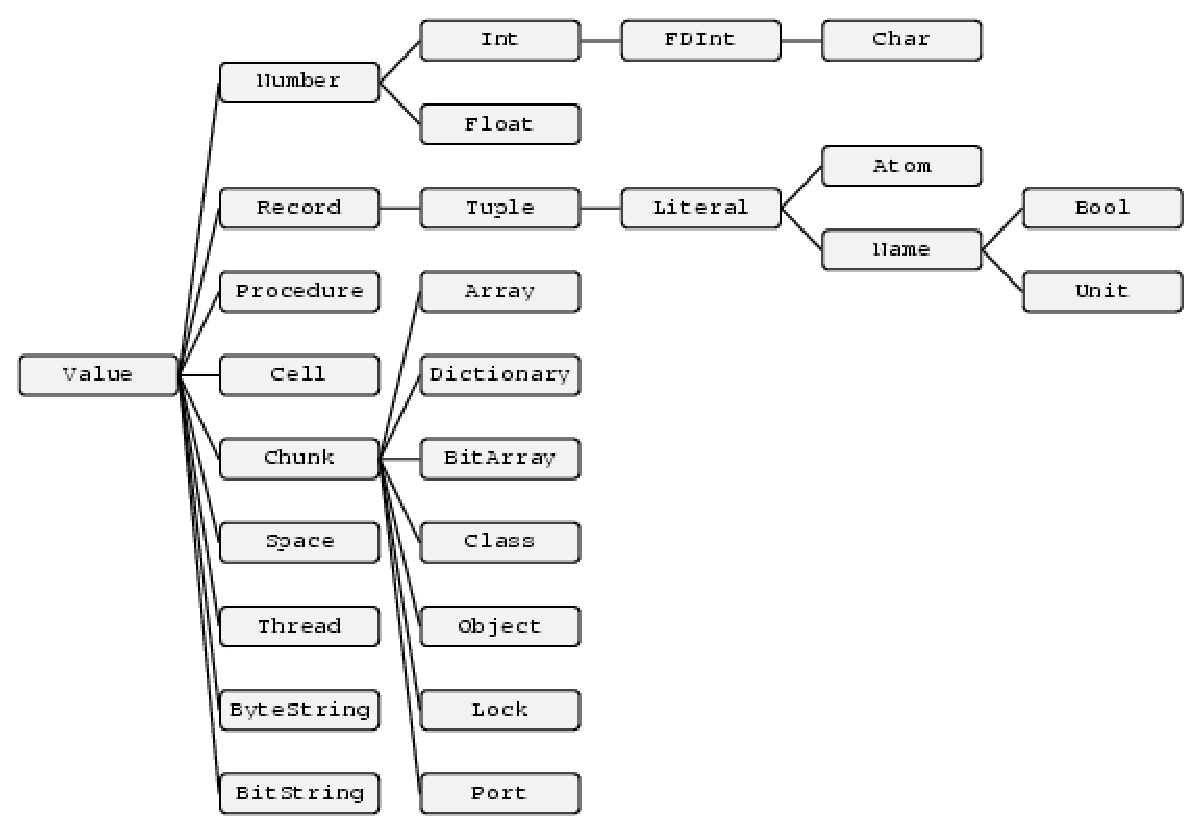
\includegraphics[width=0.70\textwidth]{../images/oz-datentypen} 
  \caption{Hierarchie der Datentypen in Oz 3. Quelle:
  \cite[Tutorial of Oz, Chapter 3.1]{url:mozart-documentation}}
  \label{fig:oz-datentypen}
\end{figure}

Einige der wichtigsten Datentypen seien hier kurz aufgeführt (vgl. 
\cite{Brunklaus:00}).

\begin{enumerate}
  \item Einfache Werte
    \begin{description}
      \item [Zahlen] können in Oz sowohl als ganze Zahlen (\texttt{Int, Char})
      als auch Fließkommazahlen (\texttt{Float}) benutzt werden.
      \item[Literale] teilen sich auf in sog. Atome und Namen. Ein Atom wird 
      durch eine alphanumerische Zeichenkette beschrieben, die entweder mit 
      einem Kleinbuchstaben beginnt oder in Hochkomma gefasst ist. Namen sind 
      eindeutige Bezeichner, die über eine spezielle Prozedur namens 
      \texttt{NewName} erzeugt werden können.
      \item[Prozeduren] können in Oz an Variablen gebunden und auch zur 
      Laufzeit erzeugt werden. \end{description}
  \item Zusammengesetzte Werte
    \begin{description}
      \item[Records] bestehen aus einem Bezeichner (Label) sowie einer festen 
      Anzahl von Komponenten oder Argumenten. Argumente bestehen aus dem Tupel 
      (Feature, Feld).
      \item[Tupel] sind ein Spezialfall von Records, bei denen die Argumente 
      kein explizites Feature besitzen.
      \item[Listen] sind eine Sonderform der Tupel. Die leere Liste wird mit
      \texttt{nil} denotiert, offene Listen bspw. als \texttt{1|2|3|nil} und 
      geschlossene Listen (also Listen mit fester Elementanzahl) als \texttt{[1 
      2 3]}.
    \end{description}
  \item \textbf{Chunks} erlauben es, abstrakte Datentypen zu konstruieren. 
  Oz bringt bereits einige vordefinierte Chunks mit, z.B. \texttt{Array} 
  oder \texttt{Dictionary}.
\end{enumerate}

\subsection{Multiparadigmisch?}
Wie bereits eingangs erwähnt, unterstützt Oz mehrere Programmierparadigmen:

\begin{enumerate}
  \item Constraint-Programmierung
  \item Funktionale Programmierung
  \item Objektorientierte Programmierung
  \item Logische Programmierung
\end{enumerate}
  
Im Gegensatz zu einer Programmiersprache, die nur eines der Paradigmen 
unterstützt, lassen sich in Oz also die zu lösenden Probleme von mehreren 
Seiten gleichzeitig mit dem jeweils geeignetsten Paradigma bearbeiten. 
Erreichen könnte man dies zwar auch durch die Kombination verschiedener 
Programmiersprachen, dabei bliebe aber der Nachteil, dass man semantische 
Lücken überwinden und Schnittstellen zwischen den einzelnen Sprachen definieren 
müsste. Dies würde u.a. zu einer aufwendigeren Fehlersuche führen. Mit Oz 
lassen sich hingegen die verschiedene Paradigmen problemlos miteinander 
kombinieren, deren gemeinsame Basis, das Oz Programming Model, im nächsten 
Abschnitt vorgestellt wird.

\subsection{Programmiermodell (Oz Programming Model, OPM)}
Die Grundlage für Berechnungen in Oz bildet das so genannte \textsl{Concurrent 
Constraint Programming}. Alle weiteren Paradigmen werden durch sog. "`syntactic 
sugar"' (Syntaxerweiterungen) in die Sprache integriert \cite{KI-LP96}.

Allgemein verwendet das Modell für Berechnungen die Metapher eines sog. 
\textsl{Berechnungsraums} (Computational Space). In diesem befindet sich zum 
einen ein \textsl{Speicher}, zum anderen eine Anzahl von sog. \textsl{Aktoren}. 
Aktoren führen die eigentlich Berechnung durch, indem sie schrittweise 
reduziert werden und sich dabei über den gemeinsamen Speicher synchronisieren. 
Dazu können Aktoren Information in den Speicher schreiben (tell) und auf 
Information warten und diese anfordern (ask).

Nebenläufigkeit (Concurrency) ist einer der wichtigsten Aspekte des OPM. Dabei 
bedeutet Nebenläufigkeit, dass verschiedene Berechnungen unabhängig voneinander 
durchgeführt werden können, nicht, dass diese parallel ablaufen.


\section{Grundlegende Techniken}
\begin{frame}{Einsatzebenen}
  \textbf{Non-Photorealistic Rendering (NPR)} kann auf drei Ebenen eingesetzt werden:
  \begin{itemize}
    \item Geometrieraum
    \item Projektionsraum
    \item Bildraum
  \end{itemize}
\end{frame}

\subsection{Techniken im Geometrieraum}
\begin{frame}{Techniken im Geometrieraum}
  \begin{itemize}
    \item direkter Einfluss auf die 3D-Geometrie der Objekte
    \item Nachteil: erfordert einen hohen Zeitaufwand
    \item wird daher selten bevorzugt
    \item Techniken:
    \begin{itemize}
      \item Computer Sketching
      \item Noise Modifier
      \item Level of Detail
    \end{itemize}
  \end{itemize}
\end{frame}

\begin{frame}{Computer Sketching}
  \begin{itemize}
    \item Paul Bourk, 1990
    \item Frage: Können CAD-Anwendungen auch unscharfe,
    an menschliche Skizzen erinnernde Entwürfe
    ausgeben?
    \item Kriterien für Skizzen:
    \begin{itemize}
      \item Linien enden nicht exakt an Schnittpunkten (Kreuzungen)
      \item Linien sind nicht gradlinig sondern "`verwackelt"'
    \end{itemize}
  \end{itemize}
\end{frame}

\begin{frame}{Computer Sketching}
  \begin{itemize}
    \item Hauptansatz: direkte Manipulation der 3D-Geometrie
    \item Umsetzung:
    \begin{itemize}
      \item Linien werden um randomisierte Faktoren verlängert
      \item Aufspalten der Linien und Mittelpunktverschiebung
    \end{itemize}
  \end{itemize}
\end{frame}

\begin{frame}{Computer Sketching}
  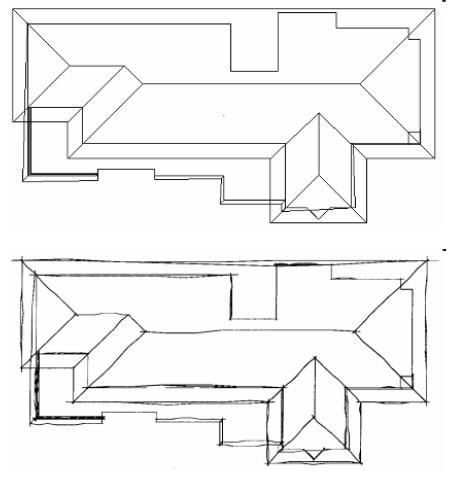
\includegraphics[width=0.5\textwidth]{../images/haus.jpg}
\end{frame}

\begin{frame}{Noise Modifier}
  \begin{itemize}
    \item "`Rauschen"' in 3D-Modellen
    \item Geometriepunkte werden um einen zufälligen Faktor
    verschoben
    \item meist Anwendung auf glatte Flächen, um
    "`natürliche"' Flächen zu erzeugen (Landschaften)
  \end{itemize}
\end{frame}

\begin{frame}{Level of Detail}
  \begin{itemize}
    \item Einsatz in vielen Bereichen:
    \begin{itemize}
      \item Kartographie: angezeigte Detailstufe in Abhängigkeit vom
      Maßstab (Generalisierung)
      \item photorealistische Darstellungen: angezeigte Detailstufe der
      Szene in Abhängigkeit von der Betrachterposition
      \item NPR: Detailstufe in Abhängigkeit zur "`Wichtigkeit"' der
      Objekte
      \begin{itemize}
        \item Eine Möglichkeit ist die Meshsimplifizierung
      \end{itemize}
    \end{itemize}
  \end{itemize}
\end{frame}

\begin{frame}{Level of Detail}
  \begin{itemize}
    \item Meshsimplifizierung:
    \begin{itemize}
      \item reduziert die Anzahl der Polygone eines 3D Modells
      \item äußere Form wird dabei approximiert
      \item Dadurch: schnellere Verarbeitung in Echtzeitsystemen möglich
    \end{itemize}
  \end{itemize}
\end{frame}

\subsection{Techniken im Projektionsraum}
\begin{frame}{Techniken im Projektionsraum}
  \begin{itemize}
    \item meistens Kombination aus Projektions- und
    Bildraumverfahren
    \item dadurch leichteres Arbeiten mit 3D-Modellen und
    Erhöhung der grafischen Qualität der Ausgabe
    \item Techniken:
    \begin{itemize}
      \item G-Buffer
      \item Line-Rendering
      \item Stroke Textures
    \end{itemize}
  \end{itemize}
\end{frame}

\begin{frame}{G-Buffer}
  \begin{itemize}
    \item "`Geometrie-Buffer"' Saito \& Takahashi, 1990
    \item in den meisten kommerziellen Cartoon-Render-Paketen implementiert
    \item Prinzip: zusätzliche Speicherung von geometrischen
    Daten zur Informationsgewinnung im Bildraum
    \begin{itemize}
      \item Flächen-Normalen des 3D-Modells
      \item UV-Koordinaten des 3D-Modells
      \item Z-Buffer des 3D-Modells
    \end{itemize}
    \item Grundidee: Informationen zur Bilderzeugung aus dem G-Buffer
    extrahieren, analysieren und zusammenfügen.  
  \end{itemize}
\end{frame}

\begin{frame}{Line-Rendering}
  \begin{itemize}
    \item Simulation der Semantik von Linien
    \item geometrische Semantik:
    \begin{itemize}
      \item Begrenzungen, Silhouetten, Diskontinuitäten (Falten)
    \end{itemize}
    \item stilistische Semantik:
    \begin{itemize}
      \item Stärke der Linien, Transparenz, Linientyp (durchgezogen,
      gestrichelt, etc.)
    \end{itemize}
  \end{itemize}
\end{frame}

\begin{frame}{Line-Rendering}
  \begin{itemize}
    \item Abspeicherung dieser zusätzlichen Attribute in
    geeigneter Form
    \begin{itemize}
      \item Eine Möglichkeit: Speicherung in Matrixform
    \end{itemize}
    \item Generierung der Attribute
    \begin{itemize}
      \item z.B. durch Inferenzregeln zu Bestimmung der
      Charakteristika der einzelnen Linien
    \end{itemize}
    \item Gute Kombinationsmöglichkeiten mit anderen
    NPR-Techniken (etwa G-Buffer)
  \end{itemize}
\end{frame}

\begin{frame}{Stroke Textures}
  \begin{itemize}
    \item Winkenbach \& Salesin, 1994
    \item Prinzip basiert auf konventionellen 2D-Malsystem
    \begin{itemize}
      \item "`strichbasierte"' Texturen werden angefertigt
      \item mittels Texturemapping auf 3D-Objekte aufgebracht
      \item Dabei: Anwendung des LOD-Prinzips auf die Textur
    \end{itemize}
  \end{itemize}
\end{frame}

\begin{frame}{Stroke Textures}
  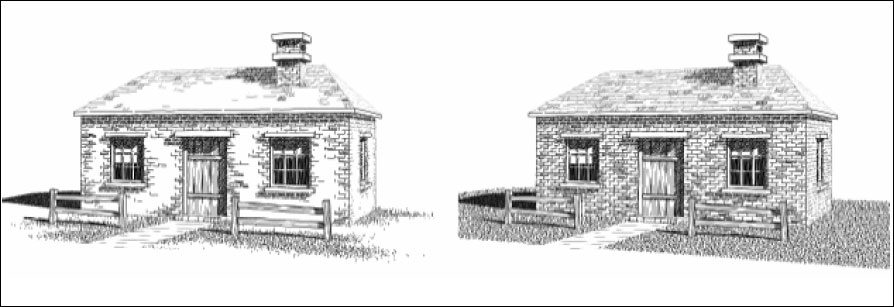
\includegraphics[width=\textwidth]{../images/strokes.jpg}
  \begin{itemize}
    \item Linienstärken und "`Detail Tags"' sind durch den
    Benutzer spezifizierbar
  \end{itemize}
\end{frame}

\subsection{Techniken im Bildraum}
\begin{frame}{Techniken im Bildraum}
  \begin{itemize}
    \item vorhandenes Bild wird analysiert und neu
    gezeichnet
    \item Techniken:
    \begin{itemize}
      \item Texture Elements
      \item Hairy brushes
      \item Iterated Function System (IFS)
    \end{itemize}
  \end{itemize}
\end{frame}

\begin{frame}{Texture Elements}
  \begin{itemize}
    \item Mezei et al., 1974
    \item Ursprünglich: Synthese sehr "`naturalistischer"' Bilder
    \item Beobachtung: in der Natur kommen sich oft
    wiederholende Muster vor
  \end{itemize}
\end{frame}

\begin{frame}{Texture Elements}
  \begin{itemize}
    \item Umsetzung: vorgefertigte grafische Subelemente
    werden zusammengefügt, um neue Bilder zu
    erzeugen
    \item Variationen durch Skalierung, Rotation und andere
    Verzerrungen
    \item Erzielt werden Verallgemeinerungen der
    Oberflächeneigenschaften, die wie menschliche
    Illustrationen wirken
  \end{itemize}
\end{frame}

\begin{frame}{Hairy Brushes}
  \begin{itemize}
    \item Strassmann, 1986
    \item Verhalten von Pinsel und Farbe soll simuliert werden
    \item Ansatz: Pinsel als 1D-Abdruck der Pinselborsten
    \item Borsten laufen an einer parametrischen Kurve
    entlang, die durch Knoten definiert ist
  \end{itemize}
\end{frame}

\begin{frame}{Hairy Brushes}
  \begin{itemize}
    \item Knoten enthalten Informationen über Position und
    Druck des Pinsels
    \item jeder "`Strich"' wird mit einer speziellen Menge an
    Farbe gezeichnet
    \item Menge nimmt mit der Länge der Linie ab
    \item erneutes "`Eintunken"' des Pinsels ist möglich
  \end{itemize}
\end{frame}

\begin{frame}{Iterated Function Systems (IFS)}
\begin{itemize}
 \item IFS: Systeme von Funktionen die wiederholt
 ausgeführt werden
 \item Einsatz: zur Beschreibung von Fraktalen
 \item Fraktale sind selbstbezüglich (rekursiv)
 \begin{itemize}
   \item Beispiel: Barnsley-Farn
     \begin{columns}
    \column{.2\textwidth}
	
\includegraphics[width=\textwidth]{../images/BarnsleyFarn.jpg}
	\column{.2\textwidth}
    
\includegraphics[width=\textwidth]{../images/BarnsleyFarnDetail.jpg}
  \end{columns}
 \end{itemize}
\end{itemize}

\end{frame}

\begin{frame}{Iterated Function Systems (IFS)}
  \begin{itemize}
    \item Nutzung des Prinzips zur fraktalen Kompression von
    Bildern (Barnsley, 1988)
    \item Kompressionstechnik basiert auf dem "`Collage-
    Theorem"' (Selbstähnlichkeit von Bildern)
  \end{itemize}
\end{frame}

\section{Einsatzgebiete}
Eine ganze Reihe von Peer-to-Peer Applikationen setzen auf der Technik von
Pastry bzw. Tapestry als zugrundeliegende Peer-to-Peer-Netzwerkinfrastruktur auf. 

\section{Tapestry in der Praxis}
Ein Beispiel für die Anwendung von Tapestry in der Praxis wäre
\textsl{OceanStore}. OceanStore ist ein global verteilter, hoch-verfügbarer
Datenspeicher. Hierbei werden die Daten des Netzwerks redundant auf den
angeschlossenen Systemen gehalten, die Zugriffe auf die jeweilig angeforderten
Daten erfolgt jeweils auf nahe Kopien. Ein weiteres, auf der Tapestry-Technik
basierendes Peer-to-Peer-System wäre \textsl{Bayeux.} Bayeux ist ein
Multicast-System, das auf die gleichzeitige Übermittlung von Multimedialen
Inhalten (Beispielsweise Audio- und Videostreams) an eine große Zahl von
Empfängern ausgerichtet ist. Ein drittes Beispiel wäre \textsl{SpamWatch.}
SpamWatch ist ein globales Spam-Filterungssystem für E-Mails, dass für alle
beteiligten Systeme Informationen über Spam-Mails publiziert.

\section{Pastry in der Praxis}
\textsl{PAST} ist ein auf Pastry basierendes verteiltes Speichersystem. Das 
Ziel von PAST ist es, Dateien in einem verteilten System so zu verteilen, dass 
man diese auch dann finden kann, wenn einzelne Knoten im Netz ausgefallen sind. 
Ein weiteres konkretes Anwendungsgebiet von Pastry ist \textsl{Scribe.} Scribe 
ist ein Kommunikationssystem, dass Nachrichten verteilt in einem 
Pastry-Netzwerk publiziert.


%\section{Wasserfarben}
\section{Wasserfarben}
\subsection{Einführung}
\begin{frame}{Einführung Wasserfarben}
  \begin{itemize}
    \item Moderne Wasserfarbentradition: zweite Hälfte des 18. Jahrhunderts
    \item Ermöglicht zahlreiche künstlerische Effekte
    \item Computer-Erzeugung durch zwei Ansätze (nach Curtis et al.): 
    realistische physikalische Simulation (hoher Aufwand) oder Annäherung durch 
    geeignete Filter (echtzeitgeeignet)
  \end{itemize}
\end{frame}

\begin{frame}{Materialien}
  \begin{itemize} 
    \item Papier: meist nicht aus Zellstoff, sondern Leinen bzw.\ Baumwolle;
    grobe Struktur, dadurch Wasserabsorption und Diffusion möglich
    \item Bestandteile der Wasserfarbe: in Wasser gelöstes Pigment, Bindemittel
    sowie Tensid (oberflächenaktiver Stoff)
    \item Pigment: festes Material, besteht aus einzelnen Partikeln; oftmals in
    Puderform; kann in das Papier einsickern und dort anhaften bzw.\ durch das
    Wasser transportiert werden
    \item Bindemittel: Pigment kann an das Papier anhaften
    \item Tensid: Wasser kann in das Papier eindringen
  \end{itemize}
\end{frame}

\begin{frame}{Haupt-Pinseltechniken}
  \begin{itemize}
    \item "`wet-on-wet painting"': Malen mit nassem, farbgetränkten Pinsel auf
    nassem Papier
    \item "`wet-on-dry painting"': Malen auf trockenem Papier
  \end{itemize}
\end{frame}

\begin{frame}{Effekte}
  \centering\pgfimage[width=1.0\textwidth]
    {../images/Curtis1997-real-watercolor-effects}
  
  \begin{itemize}
    \item \textsl{Dry-brush}: trockener Pinsel/Papier; unregelmäßige Lücken
    \item \textsl{Edge darkening}: Pigmente von innen n.\ außen; dunkle Kanten
    \item \textsl{Backruns}: Wasser läuft in nasse Region zurück
    \item \textsl{Granulation} u.\ \textsl{Separation}: körnige Struktur, Farbtrennung
    \item \textsl{Flow patterns}: freies Ausbreiten der Pinselstriche
    \item \textsl{Color glazing}: Übereinanderlegen von dünnen Farbschichten
  \end{itemize}
\end{frame}

\subsection{Computererzeugte Wasserfarben}
\begin{frame}{Simulation}
  \begin{itemize}
    \item Wichtig: nicht nur physikalische Eigenschaften, sondern auch
    künstlerische Effekte berücksichtigen!
    \item Bestandteile: Papierschicht, geordnete Menge von Farbschichten
    \item Für jede Farbschicht wird Flüssigkeitssimulation separat durchgeführt
    \item Zusätzlich: "`wet-area"'-Maske
    \item Nach der Simulation: Komposition mit Kubelka-Munk-Farbmodell erzeugt 
    finale Darstellung
  \end{itemize}
\end{frame}

\begin{frame}{Simulation: Papier}
  \begin{itemize}
    \item Vereinfachtes Papier-Modell: Textur wird als Höhenfeld und
    Flüssigkeitskapazitätsfeld abgebildet
    \item Höhe: $0 < h < 1$
    \item Steigung wird zur Berechnung der Fließgeschwindigkeit in der
    Simulation benutzt
    \item Kapazität: $c = h(c_{max} - c_{min}) + c_{min}$
  \end{itemize}
\end{frame}

\begin{frame}{Simulation: 3-Schichten-Modell}
  \begin{columns}
    \column{.6\textwidth}
	    \begin{enumerate}
	      \item "`shallow-water layer"': Wasser fließt über die Oberfläche und
	      transportiert ggf.\ Pigmente
	      \item "`pigment-deposition layer"': Pigmente werden hier abgelagert und
	      von hier weitertransportiert
	      \item "`capillary layer"': Absorbiertes Wasser diffundiert durch
	      Kapillarwirkung
	    \end{enumerate}

	\column{.4\textwidth}
		\pgfimage<3->[width=0.5\textwidth]{../images/Curtis1997-layer-shallow-water}\par
		\pgfimage<4->[width=0.5\textwidth]{../images/Curtis1997-layer-pigment-deposition}\par
		\pgfimage<5->[width=0.5\textwidth]{../images/Curtis1997-layer-capillary}
  \end{columns}
\end{frame}

\begin{frame}{Simulation: Haupt-Schleife}
  Eingabewerte: (Anfangswerte)
  \begin{itemize}
    \item Wet-Area-Maske $M$
    \item Geschwindigkeit des Wassers $u$ und $v$
    \item Wasserdruck $p$
    \item Pigmentkonzentration $g^k$
    \item Wassersättigung des Papiers $s$
  \end{itemize}
  
  \pause
  Simuliert werden über einen definierten Zeitraum: Wasser- und Pigmentbewegungen,
  Pigmentablagerungen, Kapillarfluss.
\end{frame}

\begin{frame}{Simulation: Rendering und Pigmente}
  \begin{itemize}
    \item Verwendung des Kubelka-Munk-Farbmodells
    \item Jedem RGB-Farbkanal jeden Pigments sind zwei Koeff. zugewiesen:
    \begin{itemize}
      \item Absorptionskoeff. $K$
      \item Streuungskoeff. $S$
    \end{itemize}
  \end{itemize}
  
  \begin{block}{Synthetische Pigmente}
    \pgfimage<5->[width=0.8\textwidth]{../images/Curtis1997-pigments}
  \end{block}
\end{frame}

\begin{frame}{Simulation: Vergleich der Ergebnisse}
  \centering\pgfimage[width=1.0\textwidth]
  {../images/Curtis1997-real-watercolor-effects}\par
  \centering\pgfimage[width=1.0\textwidth]
  {../images/Curtis1997-simulated-watercolor-effects}
\end{frame}

\begin{frame}{Anwendungen}
  \begin{itemize}
    \item Interaktives Malen: Benutzer kann Startzustand der Simulation
    "`malen"' durch Erstellung der Schichten mit Unterschichten für Pigmente,
    Wasser und die Wet-Area-Maske. Zusätzlich: globales Referenzbild sowie
    Papiertextur
    \item "`Watercolorization"': Konvertierung eines Farbbilds in eine
    Wasserfarben-Illustration.
    \item 3D-Szenen: Erweiterung der "`Watercolorization"'
    \item Aufbauende Ansätze: Darstellung in Echtzeit
  \end{itemize}
\end{frame}

\subsection{Echtzeit-Wasserfarben-Animationen}
\begin{frame}{Echtzeit-Animationen}
  \begin{itemize}
    \item Ansatz nach O. Deussen und T. Luft: keine exakte physikalische 
    Simulation, sondern Mittelweg zwischen Qualität und Rechenaufwand mit Ziel: 
    Echtzeit-Rendering von 3D-Szenen
    \item Aspekte: \textbf{Abstraktion und Vereinfachung},
    \textbf{Wasserfarben-Effekte}, \textbf{Licht und Schatten}
    \item Grobe Vorgehensweise: Erzeugung einzelner abstrakter 
    Wasserfarben-Layer, die mithilfe der Grafikkarte zusammengefügt werden
  \end{itemize}
\end{frame}

\subsubsection{Vorgehensweise}
\begin{frame}{Abstraktion und Vereinfachung}
  \begin{columns}[t]
    \column{0.6\textwidth}
      \begin{itemize}
        \item Jeder Layer enthält jeweils ein oder mehrere gleichartige Objekte
        \item Segmentieren der 3D-Szene anhand eindeutiger Identifikatoren
        (Ergebnis: "`intensity images"')
        \item Low-Pass-Filter erzeugt abstrakte, weiche Formen mit definierbarem
        Detaillierungsgrad
        \item Layer enthalten außerdem Farb- sowie Transparenzinformation
      \end{itemize}
    \column[T]{0.4\textwidth}
      \pgfimage<4->[width=1.0\textwidth]{../images/Luft2006-tree-segmentation}
  \end{columns}
\end{frame}

\begin{frame}{Formextraktion und Fließmuster}
  \begin{columns}[t]
    \column{0.6\textwidth}
      \begin{itemize}
        \item Form ergibt sich aus den Intensitäts-Werten der \textsl{intensity
        images}
        \item Fließmuster beschreibt das Pigment-Verhalten am Rand des Layers; 
        \textsl{wet-on-dry}: harte Kanten, \textsl{wet-on-wet}: weiche, 
        federartige Kanten
      \end{itemize}
    \column[T]{0.4\textwidth}
      \pgfimage<4->[width=1.0\textwidth]{../images/Luft2006-tree-shape-extraction-flow-pattern}
  \end{columns}
\end{frame}

\begin{frame}[label=current]{Edge darkening}
  \begin{columns}[t]
    \column{0.6\textwidth}
      \begin{itemize}
        \item Pigmente werden beim Trocknen zum Rand transportiert
        \item Imitation durch Anwendung eines Gauss-Filters, erzeugt weichen
        Intensitäts-Übergang an den Rändern
        \item Erzeugung eines Gradienten, der dem Wasserfarbenfluss folgt und
        die Transparenz an den Rändern verblassen lässt
      \end{itemize}
    \column[T]{0.4\textwidth}
      \pgfimage<4->[width=0.8\textwidth]{../images/Luft2006-tree-edge-darkening}
  \end{columns}
\end{frame}

\begin{frame}{Pigment-Granulation und Transparenz}
  \begin{columns}[t]
    \column{0.6\textwidth}
      \begin{itemize}
        \item Struktur des Papiers beeinflusst Wasserverlauf und erzeugt so Pigment-Granulation
        \item Imitation durch Verwendung einer zusätzlichen Papier-Textur
        \item Mit entsprechenden Texturen lassen sich auch ausgefranste Kanten erzeugen
      \end{itemize}
    \column[T]{0.4\textwidth}
      \pgfimage<3->[width=1.0\textwidth]{../images/Luft2006-tree-granulation-transparency}
  \end{columns}
\end{frame}

\subsubsection{Komposition von Wasserfarben-Layern}
\begin{frame}{Licht (1)}
  \begin{columns}
    \column{0.6\textwidth}
      \begin{itemize}
        \item Verwendung der Beleuchtungs-Informationen aus dem 3D-Modell zur
        Anpassung der erzeugten bzw.\ zur Erstellung neuer Layer
        \item Phong-Beleuchungsmodell, Komponenten: ambiente (hier konstant), 
        diffuse und spiegelnde Reflexion
        \item Diffuse und spiegelnde Reflexion werden auf zwei \textsl{lighting-maps} gerendert
      \end{itemize}
    \column{0.4\textwidth}
      \pgfimage<4->[width=1.0\textwidth]{../images/Luft2006-still-life-light-shadow}
  \end{columns}
\end{frame}

\begin{frame}{Licht (2)}
  \begin{columns}
    \column{0.6\textwidth}
      \begin{itemize}
        \item spiegelnde Reflexion: erzeugt hervorgehobene Region, wird erreicht
        durch Ausmaskieren der \textsl{intensity-images} vor Erstellung des
        Layers (Bild 3 und 4)
        \item diffuse Reflexion: Erzeugung zusätzlicher Layer, z.\,B.\
        Hervorhebung dunkler Stellen (Bild 3); weiterhin Anpassung aller Layer,
        zwei Farbwerte für unbeleuchtete und beleuchtete Regionen (Bild 2)
      \end{itemize}
    \column{0.4\textwidth}
      \pgfimage<2->[width=1.0\textwidth]{../images/Luft2006-still-life-light-shadow}
  \end{columns}
\end{frame}

\begin{frame}{Komposition}
  \begin{columns}[t]
    \column{0.6\textwidth}
      \begin{itemize}
        \item Layer werden mit Standard-Funktion zur Überblendung
        transparenter Objekte zusammengesetzt
        \item Farbe an der Position $(x,y)$ ergibt sich zu: $R_{rgb} = C_a \cdot
        C_{rgb} + (1-C_a) \cdot B_{rgb}$
        \item $C_{rgb}$ = Farbe, $C_a$ = Transparenz, $B_{rgb}$ = Hintergrundfarbe
      \end{itemize}
    \column[T]{0.4\textwidth}
      \pgfimage<4->[width=1.0\textwidth]{../images/Luft2006-tree-result}
  \end{columns}
\end{frame}

\begin{frame}{Demo}
  \begin{center}
	  \movie[autostart, height=6cm, width=8cm]{}{../tree_cover.avi}
  \end{center}
\end{frame}

% Schluss-Folie
\begin{frame}
  \frametitle{Danke.}
  \begin{columns}
    \column{.6\textwidth}
	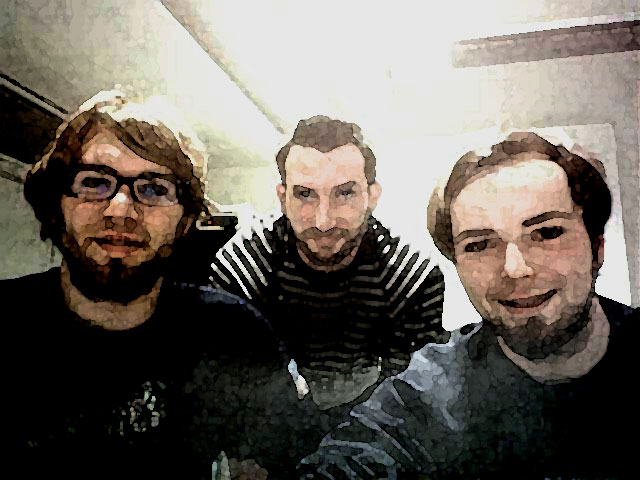
\includegraphics[width=\textwidth]{../images/wir.jpg}
	\column{.4\textwidth}
	Fragen?
  \end{columns}
\end{frame}

\end{document}